%%!TEX root=../main.tex

\section{Background}

\subsection{Dataset}
For our project, we use CCPD2019\cite{xu2018towards, li2017endtoend} as our dataset. 
CCPD is a projects refers to Chinese City Parking Dataset which consists 
nearly 300 thousand Chinese licence plate pictures which is recently updated in 2019.
The dataset are collected from several parking lots in China, 
and the collecting time was from 7:30 a.m to 10:00 p.m. 
All pictures are taken with a handheld Android device. An example is shown in Figure \ref{fig:02_example}.
The dataset involves a variety of complex light and weather conditions 
including blurry, rainy and snowy and the dimension of each image is 720 x 
1160 with RGB color (3 channels).

In this dataset, the annotations of each images is in their respective file name. The 
meta info is being leveraged to help us built a more robust system. The 2 most crucial 
data pieces are the four vertices forming around the bounding box and
the license plate value encoding according the their custom encoding format.

\begin{figure}
\centering
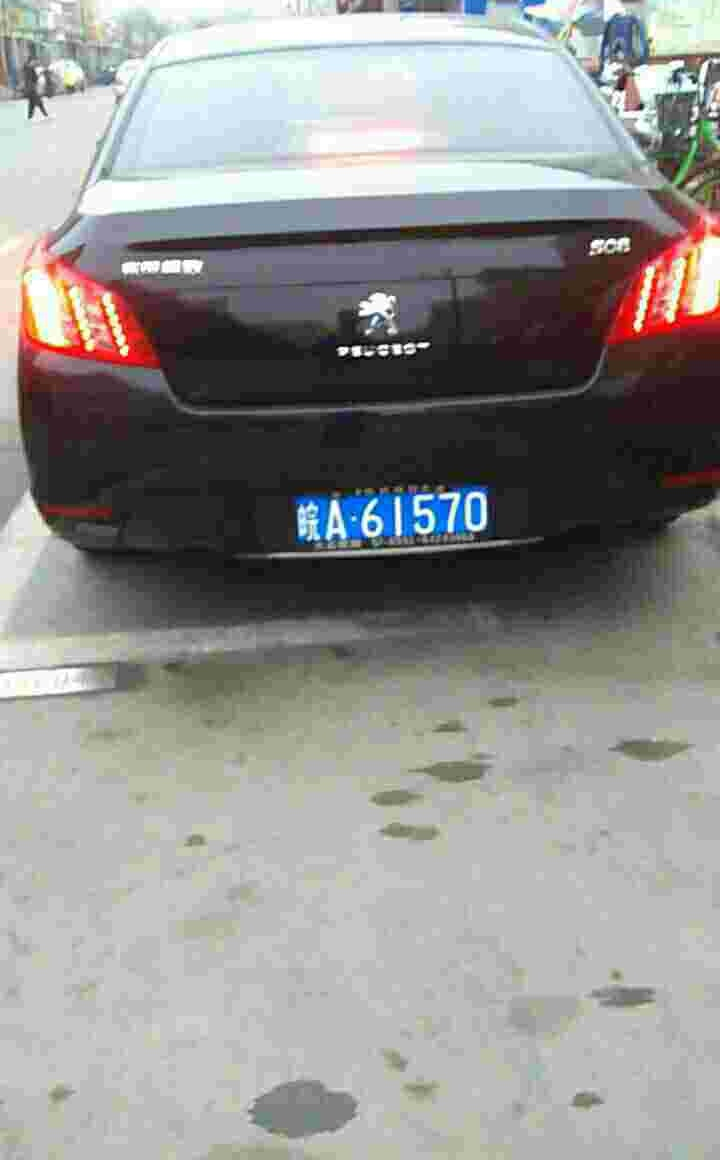
\includegraphics[width=2.5in]{\FIGDIR/02_example.jpg}
\caption{Example of an original image from the data set}
\label{fig:02_example}
\vspace{-0.25in}
\end{figure}

\subsection{Licence Plate detection algorithm}
There are mainly 2 ways to employ licence plate detection which is the 
traditional contour detection methods and Neural Network based methods 
such as YOLO\cite{redmon2015look}.

Traditional methods \cite{lpdectionComplex, NovelLPDectionWavelet,LPDetectMultiStage}, 
leverage some common techniques of image processing, including but not limit to edge detection, 
de-noising, feature extraction to calculate the location the licence plate in the image.

% EXPAND if needed
By introducing the morphology method\cite{lpdectionComplex} to reduce the number 
of candidates significantly allows speeding up the process of plate detection. 
A wavelet transform based method\cite{NovelLPDectionWavelet} and a empirical 
mode decomposition analysis can also be used to detect the licence plate
On top of that, detection can also be done by extracting a background color of
the license plate as a crucial feature\cite{LPDetectMultiStage, DPLHSIcolor}.

For this project, the major focus is the follow-up stage on the plate character
recognition. Therefore, we have developed a relatively simple plate detection
algorithm having 6 stages:
\begin{enumerate}
    \item Converting RGB-colored images to gray-scale images 
    \item Smoothing and de-noising are applied to the gray-scale images
    \item Employing a Sobel\-Feldman operator\cite{SobelOp} to perform edge detection
    \item Extracting the edges and Converting the gray-scale images into binary images
    \item Filtering out the unrelated background area to create bounding area around the plate
    \item Segmenting the plate area into individual characters
\end{enumerate}
After the images have gone through the pre-processing steps, we can then further 
apply CNN-based techniques for character recognition. 
Also, we can then "learn" the dictionary for sparse encoding and solve for the representation
for the images which more detail will be discussed in the following sections.

\subsection{Sparse Representation}
Sparse representation\cite{SpareRepre} has now become a new norm in image, signal
and computational imaging. The core idea behind this successive approach is the 
reconstruction of a signal $s$ from a sparse representation $x$ according to a 
linear dictionary matrix $D$ so $Dx$ is approximately equals to $s$\cite{CDLreview2018}. 
Instead of using the original signal, which is usually larger in memory size, we can then 
pass the sparse representation to neural-network based approach for further processing.

There are two major challenges using this kind of approach
\begin{enumerate}
    \item How to construct a the linear dictionary $D$?
    \item How to solve for the sparse representation $x$ from $D$?
\end{enumerate}

In the earlier stage of the sparse representation, fixed-base dictionary 
combining multiple linear filters are used\cite{5452966}. 
The advantage of this approach is that we don't need
any inputs or training set to develop the dictionary. However, the disadvantage
are obvious that a one-size-fit-all approach is not going to give us the 
optimal result. On top of that, the quality of final sparse representation 
heavily depends on the dictionary it is based on. Luckily more recent researches
have proposed methods to "learn" a dictionary from a set of training approaches.

To solve for a suitable sparse coding, many researches have pointed toward
algorithms that is based on Alternating Direction Method of Multipliers
(ADMM)\cite{CDLreview2018}. ADMM's 2 main features are the decomposition 
of the problem into 2 stages and exploitation of the FFT for computational 
advantage.

Since we are mainly dealing with 2D images of license plates, the dictionary Learning
and sparse coding problem being discussed will be in the convolution variant namely,
Convolution Dictionary Learning (CDL) and Convolution Sparse Coding (CSC).

\subsection{Convolution Dictionary Learning (CDL)}
There are 3 main CDL variants we want to explore in this paper:
\begin{enumerate}
    \item CDL with ADMM update\cite{SOREL201644}
    \item CDL with ADMM consensus update\cite{SOREL201644,CDLreview2018}
\end{enumerate}

\paragraph{CDL with ADMM update}
A very simple summary of the ADMM framework proposed is provided below:
\begin{enumerate}
    \item Use shrinkage or soft thresh-holding to solve for the penalty parameter
    \item Use Fast Fourier Transform (FFT) to deal with computationally expensive convolution
    operation
\end{enumerate}

\paragraph{CDL with ADMM consensus update}
Consensus update allows the images to be feed to the ADMM framework in a 
batch mode due to the introduction of different block matrix for mapping 
coefficient. This methods can reduce the time needed to solve for the 
dictionary.

\subsection{Convolution Sparse Coding (CSC)}
There are 3 main CSC variants that are explored in this paper:
\begin{enumerate}
    \item Single-channel CSC
    \item FISTA CBPDN Solver
\end{enumerate}
Since the final image used for CDL and CSC are gary-scale images
with one channels, most the the CSC algorithms chosen is single channel.
The major formulation of CSC is shown below:
\begin{equation}
    \mathrm{argmin}_\mathbf{x} \; \frac{1}{2} \left\| \sum_m \mathbf{d}_m * \mathbf{x}_{m} - \mathbf{s} \right\|_2^2 + \lambda \sum_m \| \mathbf{x}_{m} \|_1 \;,
\end{equation}

\paragraph{Single-channel CSC}
The most basic form of a sparse coding algorithm based on
the standard Basis Pursuit DeNoising(BPDN). The convolution 
form of the BPDN is called Convolution BPDN (CBPDN) 

\paragraph{FISTA CBPDN Solver}
This variant incorporates the use of the Fast Iterative 
Shrinkage-Thresholding Algorithm (FISTA) which is an accelerated
proximal gradient method.

